\title{CS 311, Assignment 0 - Report} % You may change the title if you want.
% \subtitle{Hello}
\author{Abhishek Raj (180010002), Harsh Raj (180010027), Rishit Saiya (180010027)}

\date{\today}

\documentclass[12pt]{article}
\usepackage{fullpage}
\usepackage{enumitem}
\usepackage{amsmath,mathtools}
\usepackage{amssymb}
\usepackage[super]{nth}
\usepackage{textcomp}
\usepackage{hyperref}
\begin{document}
\maketitle

%---------------------------------------------------------------------

\section{Abstract}
The report touches upon the algorithmic approaches used varying different parameters like width, probability of Sensors being ON, etc. to achieve the motive of infiltrator during the course of progress from AC (Attacking Country) to DC (Defending Country).
It also explains in details our previous versions/ideas and the breakpoints where we chose a different idea to enhance and achieve the results.

%---------------------------------------------------------------------

\section{Assumptions \& Trivial Parameters}
In accordance with the description of the challenge, the length has to be infinitely long. So, the length we have chosen is as follows:

\begin{equation*}
    L = 1000
\end{equation*}

From the challenge description, the sensor is switched \textbf{ON}, if we receive \textbf{Heads} in the coin toss, which in turn depends upon the array/spectrum of probabilities we are considering.
The following Set $P$ represents the set containing the probabilities of sensors being ON we have considered:
\begin{equation*}
    P = \{0.2, 0.3, 0.4, 0.5, 0.6, 0.8\}
\end{equation*}
WLOG, the time taken by the infiltrator to reach DC from AC will increase if width is increased. The following Set $W$ represents the set of width we considered for pairing with $P's$ elements to understand and comprehend on different time results.
\begin{equation*}
    W = \{4, 6, 10, 12, 16, 20, 24, 30\}
\end{equation*}
The infiltrator only moves ahead from AC to DC and no step backwards it taken. With a time span of every 10 secs, a coin is tossed and based on that upcoming step from the neighbouring 8 is chosen.

%---------------------------------------------------------------------

\section{Deductions}

\begin{itemize}
    \item \textbf{Effect due to variation in width} \\
    As the parameter ‘w’ (width) was increased, the time taken by the infiltrator to cross from DC to AC also increased. The reason behind that is that, the infiltrator will have to cover more distance with increasing value of width.
    \item \textbf{Effect due to variation of probability of sensors being ON} \\
    As the probability of sensors being ON increased, the time taken by the infiltrator to cross also increases. The reason behind that is that, as the probability of sensors being ON increases, the infiltrator's options to proceed towards DC diminishes and hence time required will increase.
\end{itemize}

Given the above 2 statements are taken under consideration, our algorithms and optimization are based on the same notion over developing it. The 3-D graph in Figure 1 depicts average time variation over width and probabilities.
%---------------------------------------------------------------------

\section{Approach \& Code}
For the above given sets of $P$ \& $W$, we tried all cross combinations i.e. for a given $P$, we tried all $W's$ with it and found out all different times. However to normalize the time taken for a given pair of (P,W) for 50 iterations, we just took average of all times.

%---------------------------------------------------------------------

\section{Code, Compilation \& Execution}
A clean and readable code formation system is used. We have created 5 main files of codes which are as follows:
    \begin{itemize}
        \item Border.java
        \item Clock.java
        \item Coin.java
        \item Infiltrator.java
        \item Main.java
        \item Sensor.java
    \end{itemize}

Each file is embedded with a separate class which finally top inherits to \textit{Main.java} file. The command line executions are: \\
$>>$ \textit{javac .*} \\
$>>$ \textit{java Main input.txt output.txt} \\ 

It is to be noted that \textbf{\textit{input.txt}} contains the sets $P$ \& $W$.
\\


The \textbf{\textit{output.txt}} gives the following results: 


($P_i$) ($W_i$) (Average time of 50 iterations of \{$P_i$,$W_i$\})
\\

Additionally, we have made a file called \textbf{\textit{graph\_plotter.py}} for plotting graph using Matplotlib libraries in Python. Further explanation and deductions are given in below section.
%---------------------------------------------------------------------

\section{Graph}
Figure 1 shows the graph and where we have used the parameters as follows:
\begin{itemize}
    \item X-Axis: Width
    \item Y-Axis: Probability
    \item Z-Axis: Time
\end{itemize}

The graph just depicts and proves the deductions which we made above.
\begin{center}
    \begin{figure}
        \centering
        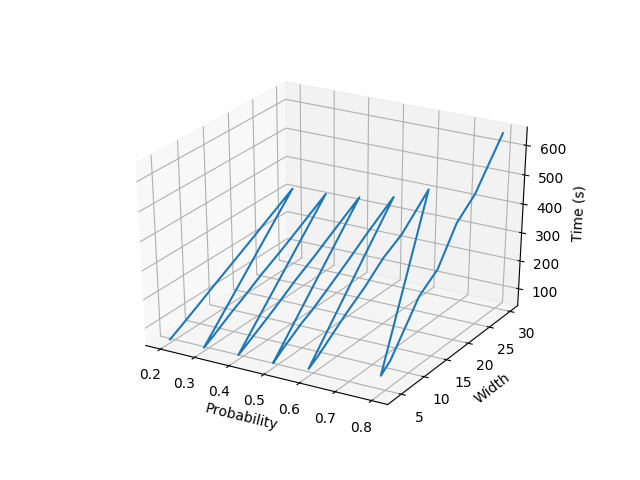
\includegraphics[width=15cm, height=10cm]{graph.png}
        \caption{Variation of Probability, Width and Average Time}
    \end{figure}
\end{center}

\end{document}